\def\mytitle{LINE ASSIGNMENT}
\def\myauthor{Uday Kumar}
\def\contact{immadisettyudaykumar15@gmail.com}
\def\mymodule{Future Wireless Communication (FWC)}
\documentclass[10pt, a4paper]{article}
\usepackage[a4paper,outer=1.5cm,inner=1.5cm,top=1.75cm,bottom=1.5cm]{geometry}
\twocolumn
\usepackage{graphicx}
\graphicspath{{./images/}}
\usepackage[colorlinks,linkcolor={black},citecolor={blue!80!black},urlcolor={blue!80!black}]{hyperref}
\usepackage[parfill]{parskip}
\usepackage{lmodern}
\usepackage{tikz}
% \usepackage{physics}
%\documentclass[tikz, border=2mm]{standalone}
%\usepackage{karnaugh-map}
%\documentclass{article}
\usepackage{tabularx}
\usepackage{circuitikz}
\usetikzlibrary{calc}
\usepackage{amsmath}
\usepackage{amssymb}
\renewcommand*\familydefault{\sfdefault}
\usepackage{watermark}
\providecommand{\norm}[1]{\left\lVert#1\right\rVert}
\usepackage{lipsum}
\usepackage{xcolor}
\usepackage{listings}
\usepackage{float}
\usepackage{titlesec}
\providecommand{\mtx}[1]{\mathbf{#1}}
\titlespacing{\subsection}{1pt}{\parskip}{3pt}
\titlespacing{\subsubsection}{0pt}{\parskip}{-\parskip}
\titlespacing{\paragraph}{0pt}{\parskip}{\parskip}
\newcommand{\figuremacro}[5]{
    \begin{figure}[#1]
        \centering
        \includegraphics[width=#5\columnwidth]{#2}
        \caption[#3]{\textbf{#3}#4}
        \label{fig:#2}
    \end{figure}
}
\newcommand{\myvec}[1]{\ensuremath{\begin{pmatrix}#1\end{pmatrix}}}
\let\vec\mathbf
\lstset{
frame=single, 
breaklines=true,
columns=fullflexible
}

\title{\mytitle}
\author{\myauthor\hspace{1em}\\\contact\\FWC22086\hspace{6.5em}IITH\hspace{0.5em}\mymodule\hspace{6em}MATRICES}
\date{}
\begin{document}
 \maketitle
 \paragraph*{\large Problem Statement}
$-$ \textbf{ A straight line L is perpendicular to the line 5x-y=1.The area of the triangle formed by the line and the coordinate axis is 5.Find the equation of line L.}
 
\begin{figure}[h]
\centering
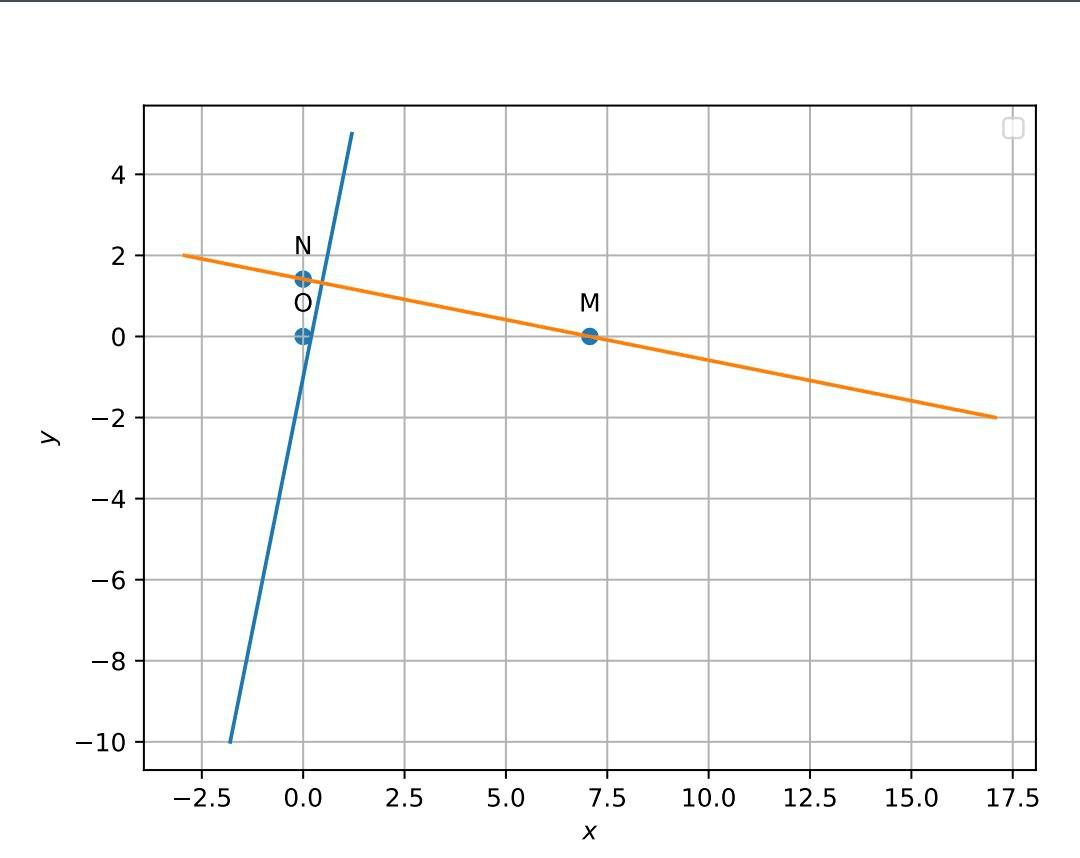
\includegraphics[width=1\columnwidth]{linedg.png}
\caption{Perpendcular line}
\end{figure}
 \section*{Construction}
\vspace{2mm}
 The input parameters are as follows
{
\setlength\extrarowheight{4pt}
\begin{center}
 \begin{tabular}{|c|c|c|}
 \hline
 \textbf{Symbol}&\textbf{Value}&\textbf{Description}\\
 \hline
 $\vec{n_1}$&$
 \begin{pmatrix}
  5\\
  -1\\
 \end{pmatrix}$
 &normal vector \\
 \hline
 $c_1$&$
 \begin{pmatrix}
  1\\
 \end{pmatrix}$
 &constant\\
 \hline
 $\vec{n_2}$&$
 \begin{pmatrix}
  1\\
  5\\
 \end{pmatrix}$
 &direction vector\\
 \hline
 $e_1$&$
 \begin{pmatrix}
  1\\
  0\\
 \end{pmatrix}$
 &\\
 \hline
 $e_1$&$
 \begin{pmatrix}
  1\\
  0\\
 \end{pmatrix}$
 &\\
 \hline
 M&$
 \begin{pmatrix}
  a\\
  0\\
 \end{pmatrix}$
 &$$$e_1$$^T\vec{(a)}$ \\
 \hline
 N&$
 \begin{pmatrix}
  0\\
  b\\
 \end{pmatrix}$
 &$$$e_2$$^T\vec{(b)}$\\
 \hline
 \end{tabular}
 \end{center}
}
\section*{\large solution}

\subsection*{\large step 1}
let the given equation is 
\begin{eqnarray}
	\vec{n_1^T}\myvec{x}=c
\end{eqnarray}
\\Direction vectors of the perpendicular line is
\begin{eqnarray}                                   \vec{n_1^T}\vec{n_2}=0              
\end{eqnarray}
\begin{equation}
\vec{n_2}=\myvec{1\\5}
\end{equation}
\\The  perpendicular line meets the coordinate axis at two points and forms a triangle with area Q=5
\\
Let the two points be M,N and O is the origin
\\
\\The two points lies on the line with direction vector m ,we get the condition
\begin{eqnarray}
\vec{n_2^T\vec{(M)}}=\vec{n_2^T\vec{(N)}}
\end{eqnarray}
%\\Equation of the passing through M is 
%\begin{eqnarray}
% (1\;5)\myvec{x-a\\y-0}=0
%\end{eqnarray}
%\\Equation of the line passing through N is 
%\begin{eqnarray}
% (1\;5)\myvec{x-0\\y-b}=0
%\end{eqnarray}
\\Solving the above two equations we get
\begin{center}
a = 5b
\end{center}
\
\\substitute a=5b then the points become
\begin{center}
\begin{equation}
\vec{M}=\myvec{5b\\0} \vec{N}=\myvec{0\\b}
\end{equation}
\end{center} 
\
\\To find the value of b
\\Given the area of the triangle formed by the points OMN is Q
\begin{equation}
\vec{V_1}=\vec{O}-\vec{M},
\vec{V_2}=\vec{O}-\vec{N}
\end{equation}
\begin{center}
\textbf{$$ \frac{1}{2}\norm{(\vec{V_1}) \times  (\vec{V_2})} =Q  $$} 
\end{center}\label{eq-7}
\
\\by solving we get 
\begin{center}
b = $\sqrt{2}$
\end{center} 
\
\\To get the value of  $c_2$
\begin{eqnarray}
\vec{n_2^T}\myvec{M}=c_2
\end{eqnarray}
we get
\begin{center}
$c_2$=5$\sqrt{2}$
\end{center}
\begin{center}
\end{center}
The final equation is
\begin{eqnarray}
 \vec{n_2^T}\myvec{x}=c_2
\end{eqnarray}
\end{document}
